\label{corpus}
\minitoc
\section{Description du corpus Charcot}
Le fonds patrimonial de Jean-Martin Charcot est conservé à la Bibliothèque de Neurosciences Jean-Martin Charcot par la BSU.
%\footnote{\url{https://www.sorbonne-universite.fr/bu/decouvrir-nos-bibliotheques/la-bibliotheque-charcot}.}
 Ce fonds regroupe des ouvrages suivants : 
\begin{itemize}
\item fonds historique Charcot (bibliothèque personnelle de Charcot) : ouvrages, périodiques, collection de thèses et de tirés à part, manuscrits, observations, collection neurologique couvrant la seconde partie du XIX\ieme{} siècle, fonds bibliophilique ancien ;
\item collections de la bibliothèque des Internes de la Salpêtrière : ouvrages, périodiques, thèses en neurologie et psychiatrie pour la période 1800-1950 ;
\item donations en ouvrages du docteur Achille Souques.
\end{itemize}
\medskip
Dans un souci de préservation d'ouvrages originaux et de valorisation de collections ayant un caractère iconographique notable, une partie de ce fonds a été numérisée. Ces archives numérisées sont disponibles sur le portail numérique
SorbonNum\footnote{anc. Jubilothèque, \url{https://patrimoine.sorbonne-universite.fr/collection/Fonds-Charcot}}, porte d'entrée unique vers les collections scientifiques patrimoniales et numériques de Sorbonne Université, ainsi que sur Gallica, bibliothèque numérique de la Bibliothèque nationale de France (\textsc{BnF})\footnote{\url{https://gallica.bnf.fr/services/engine/search/sru?operation=searchRetrieve&version=1.2&query=\%28gallica\%20all\%20\%22Charcot\%2C\%20Jean-Martin\%22\%29&lang=fr&suggest=0}.}.

Le fonds numérisé a été décrit et divisé par la BSU en quatre grandes typologies de documents :
\begin{enumerate}
\item \underline{Fonds iconographique}
\begin{itemize}
\item \textbf{Album des internes} : Album des promotions annuelles d'internes, photographiées et classées par établissements de l'Assistance Publique, entre 1860 et 1963 ;
\item \textbf{Photographies sur les aliénés de Bicêtre par Désiré Magloire Bourneville} : deux albums présentant les photographies des \og{}petits enfants anormaux\fg{} hospitalisés à Bicêtre dans le service du docteur Bourneville, collaborateur de Charcot.
\end{itemize}
\item \underline{Leçons et manuscrits des leçons de Charcot}
\begin{itemize}
\item \textbf{Manuscrits des leçons et observations de Charcot (1825-1893)} : leçons orales de Charcot, rédigées intégralement de sa main et annotées ;
\item \textbf{Leçons de Charcot} : numérisation des volumes de l'\textit{\OE{}uvre Complète} de Charcot consacrés au système nerveux et à l'enseignement clinique, comme par exemple les célèbres leçons du Mardi, sur l'hystérie notamment.
\end{itemize}
\item \underline{Périodiques}
\begin{itemize}
\item \textbf{\textit{Les Recherches cliniques et thérapeutiques sur l'épilepsie, l'hystérie et l'idiotie (1872 -1903)}} de Bourneville. Y est retracée toute l'activité du Service des Enfants Idiots, à la Salpêtrière puis à Bicêtre, par le biais des compte-rendu illustrés de photographies et rédigés par Bourneville ;
\item \textbf{\textit{Revue de l'Hypnotisme (1887-1910)}} : périodique consacré à l'hypnotisme que Charcot a réhabilité, publiant les principaux articles théoriques sur cette discipline ;
\item \textbf{\textit{Journal du magnétisme (1845-1861)}} : la collection reflète les recherches sur le magnétisme, renouvelées au milieu du XIX\ieme{} siècle ; 
\item \textbf{\textit{Revue photographique des hôpitaux de Paris (1869-1872)}}. Première revue exposant les applications de la photographie à la médecine, notamment la médecine hospitalière, à travers les études menées à l'Hôpital Saint Louis, et à la Salpêtrière ;
\item \textbf{\textit{Iconographie Photographique de la Salpêtrière (1875-1879)}}. La collection présente les observations de patientes examinées à la Salpêtrière, accompagnées de photographies d'Albert Londe, présentant les divers stades de la crise d'hystérie ;
\item \textbf{\textit{Nouvelle Iconographie de la Salpêtrière (1888-1918)}}. La revue est fondée sous la direction de Charcot par Paul Richer, Gilles de la Tourette et Albert Londe, directeur du service photographique. Elle réunit la collection de clichés constituée à la Salpêtrière a pour but la représentation objective des pathologies observées. Elle prend la relève de l'\textit{Iconographie Photographique de la Salpêtrière}. Les articles sont illustrés de photographies, de dessins et de lithographies ;
\item \textbf{\textit{Archives de neurologie (1880-1907)}}. Sous-titrée \og{}Revue trimestrielle des maladies nerveuses et mentales\fg{}, les Archives de neurologie sont publiées sous la direction de Charcot par Bourneville. La revue édite, groupe, catégorise et compare la masse des travaux de pathologie nerveuse. Les \textit{Archives de neurologie} sont devenues bisannuelles en 1881.
\end{itemize}
\item \underline{Ouvrages de la bibliothèque de Charcot}
\begin{itemize}
\item \textbf{Collection d'atlas d'anatomie et de pathologie du système nerveux}, publiés durant le XIX\ieme{} siècle. L'iconographie de ces ouvrages est remarquable, à commencer par l'\textit{Atlas de Vicq d'Azyr}, médecin du roi Louis XVI ;
\item \textbf{Traités}. Cette collection regroupe à la fois des traités sélectionnés dans la bibliothèque de Charcot (comme l'\textit{Opera omnia}$\dots$ de Thomas Willis, 1682, comportant des gravures), des atlas et des textes significatifs des successeurs de Charcot, issus de la bibliothèque des Internes de la Salpêtrière (par exemple l'\textit{Anatomie des centres nerveux} des Déjerine).
\end{itemize}
\end{enumerate}



\section{Constitution du corpus Charcot}
Le corpus de travail est constitué de 201 documents OCRisés, sans post-correction, gracieusement fournis au format \textsc{XML} par la \textsc{BSU}\footnote{À cette occasion, je remercie chaleureusement M\textsuperscript{me} Adeline Batailler, chargée de la valorisation et de l'évaluation des collections du département des Collections de la \textsc{BSU}, pour ses conseils précieux concernant le fonds Charcot.}. Originalement, ces fichiers ne contenaient que les balises \texttt{<doc>} (document comme objet), \texttt{<id\_doc>} (identifiant du document) et \texttt{<pages>} (pages du document), raison pour laquelle nous avons procédé, dans un premier temps, à une restructuration des textes en \textsc{XML-TEI} à l'aide de l'outil \textsc{Teinte}\footnote{\url{https://github.com/OBVIL/teinte\_obtic}}, afin de permettre la fouille avancée du corpus Charcot à travers des outils développés au sein de l'équipe-projet \textsc{ObTIC}. D'une part, le moteur de recherche \textsc{OBVIE}\footnote{\url{https://obtic.huma-num.fr/obvie/}. Pour d'amples informations sur le fonctionnement de cet outil, \textit{cf}. \citet{alrahabi2022obvie}.} permet de repérer des textes similaires par ordre de pertinence à partir des termes en commun. D'autre part, l'algorithme \textsc{TextPair} génère une liste de passages similaires, c'est-à-dire les séquences de mots qui se chevauchent (n-grammes de mots) pour chaque texte, en comparant ensuite ces résultats avec ceux de séquences dans d'autres textes\footnote{\url{https://artfl-project.uchicago.edu/text-pair.}}.

Afin de mesurer l'impact de Charcot sur son entourage et d'analyser la circulation de concepts véhiculés dans le corpus, nous avons commencé par séparer les documents rédigés par Charcot de ceux rédigés par ses co-auteurs (p. ex. Bourneville) ou les auteurs thématiquement proches de lui (p. ex. de la Tourette). Nous avons obtenu respectivement 68 (corpus \og{}Charcot\fg{}) et 133 (corpus \og{}Autres\fg{}) documents, comme présenté dans le tableau \ref{tab:corpus}. 

\begin{table}[!ht]
    \centering
    \begin{tabular}{|c|r|r|c|}
    \hline\hline
    \rowcolor{gray!10}
    \small
       Corpus & \multicolumn{1}{c|}{\begin{tabular}[c]{@{}c@{}}\small Nombre \vspace{-0.20cm} \\ \small de documents\end{tabular}} & \multicolumn{1}{c|}{\begin{tabular}[c]{@{}c@{}}\small Nombre de tokens\end{tabular}} & {\begin{tabular}[c]{@{}c@{}}\small Mémoire\end{tabular}} \\ \hline
   
      \begin{tabular}[c]{@{}c@{}}\textrm{\small Charcot}\\ \scriptsize{textes rédigés par Charcot}\end{tabular}  & \small 68 & \small 12 190 649 (38,12 \%) & {\begin{tabular}[r]{@{}c@{}}\small 79,1 Mo\end{tabular}} \\ \hline
      
       \begin{tabular}[c]{@{}c@{}}\textrm{\small Autres}\\\vspace{-0.15cm} \scriptsize{textes rédigés par les membres} \vspace{-0.15cm} \\ \scriptsize{de son réseau scientifique}\end{tabular}    & \small 133 & \small 19 788 830 (61,88 \%) & {\begin{tabular}[r]{@{}c@{}}\small 127,2 Mo\end{tabular}} \\
       \hline\hline
       \textbf{TOTAL} & \textbf{201} & \textbf{31 979 479} (100 \%) & \textbf{206,3 Mo}\\
       \hline\hline
    \end{tabular}
    \caption{Répartition du fonds Charcot selon les auteurs.
%    \footnote{\tiny{\url{https://patrimoine.sorbonne-universite.fr/collection/Fonds-Charcot}}}
}
 \label{tab:corpus}
\end{table}

Les deux corpus issus du fonds Charcot sont librement disponibles et interrogeables sur les deux plateformes \textsc{OBVIE}\footnote{\url{https://obtic.huma-num.fr/obvie/charcot/?view=corpus}} et \textsc{TextPair}\footnote{\url{https://anomander.uchicago.edu/}}.

dépôt GitHub avec les données\footnote{\url{https://github.com/ljpetkovic/Charcot_circulations/tree/main/input}}
\hl{métadonnées sur les deux corpus...}

\hl{Répartition des \oe{}uvres sur les années : chronologiquement, cf. le graphique généré au SCAI}

\begin{figure}[h]
	\centering
	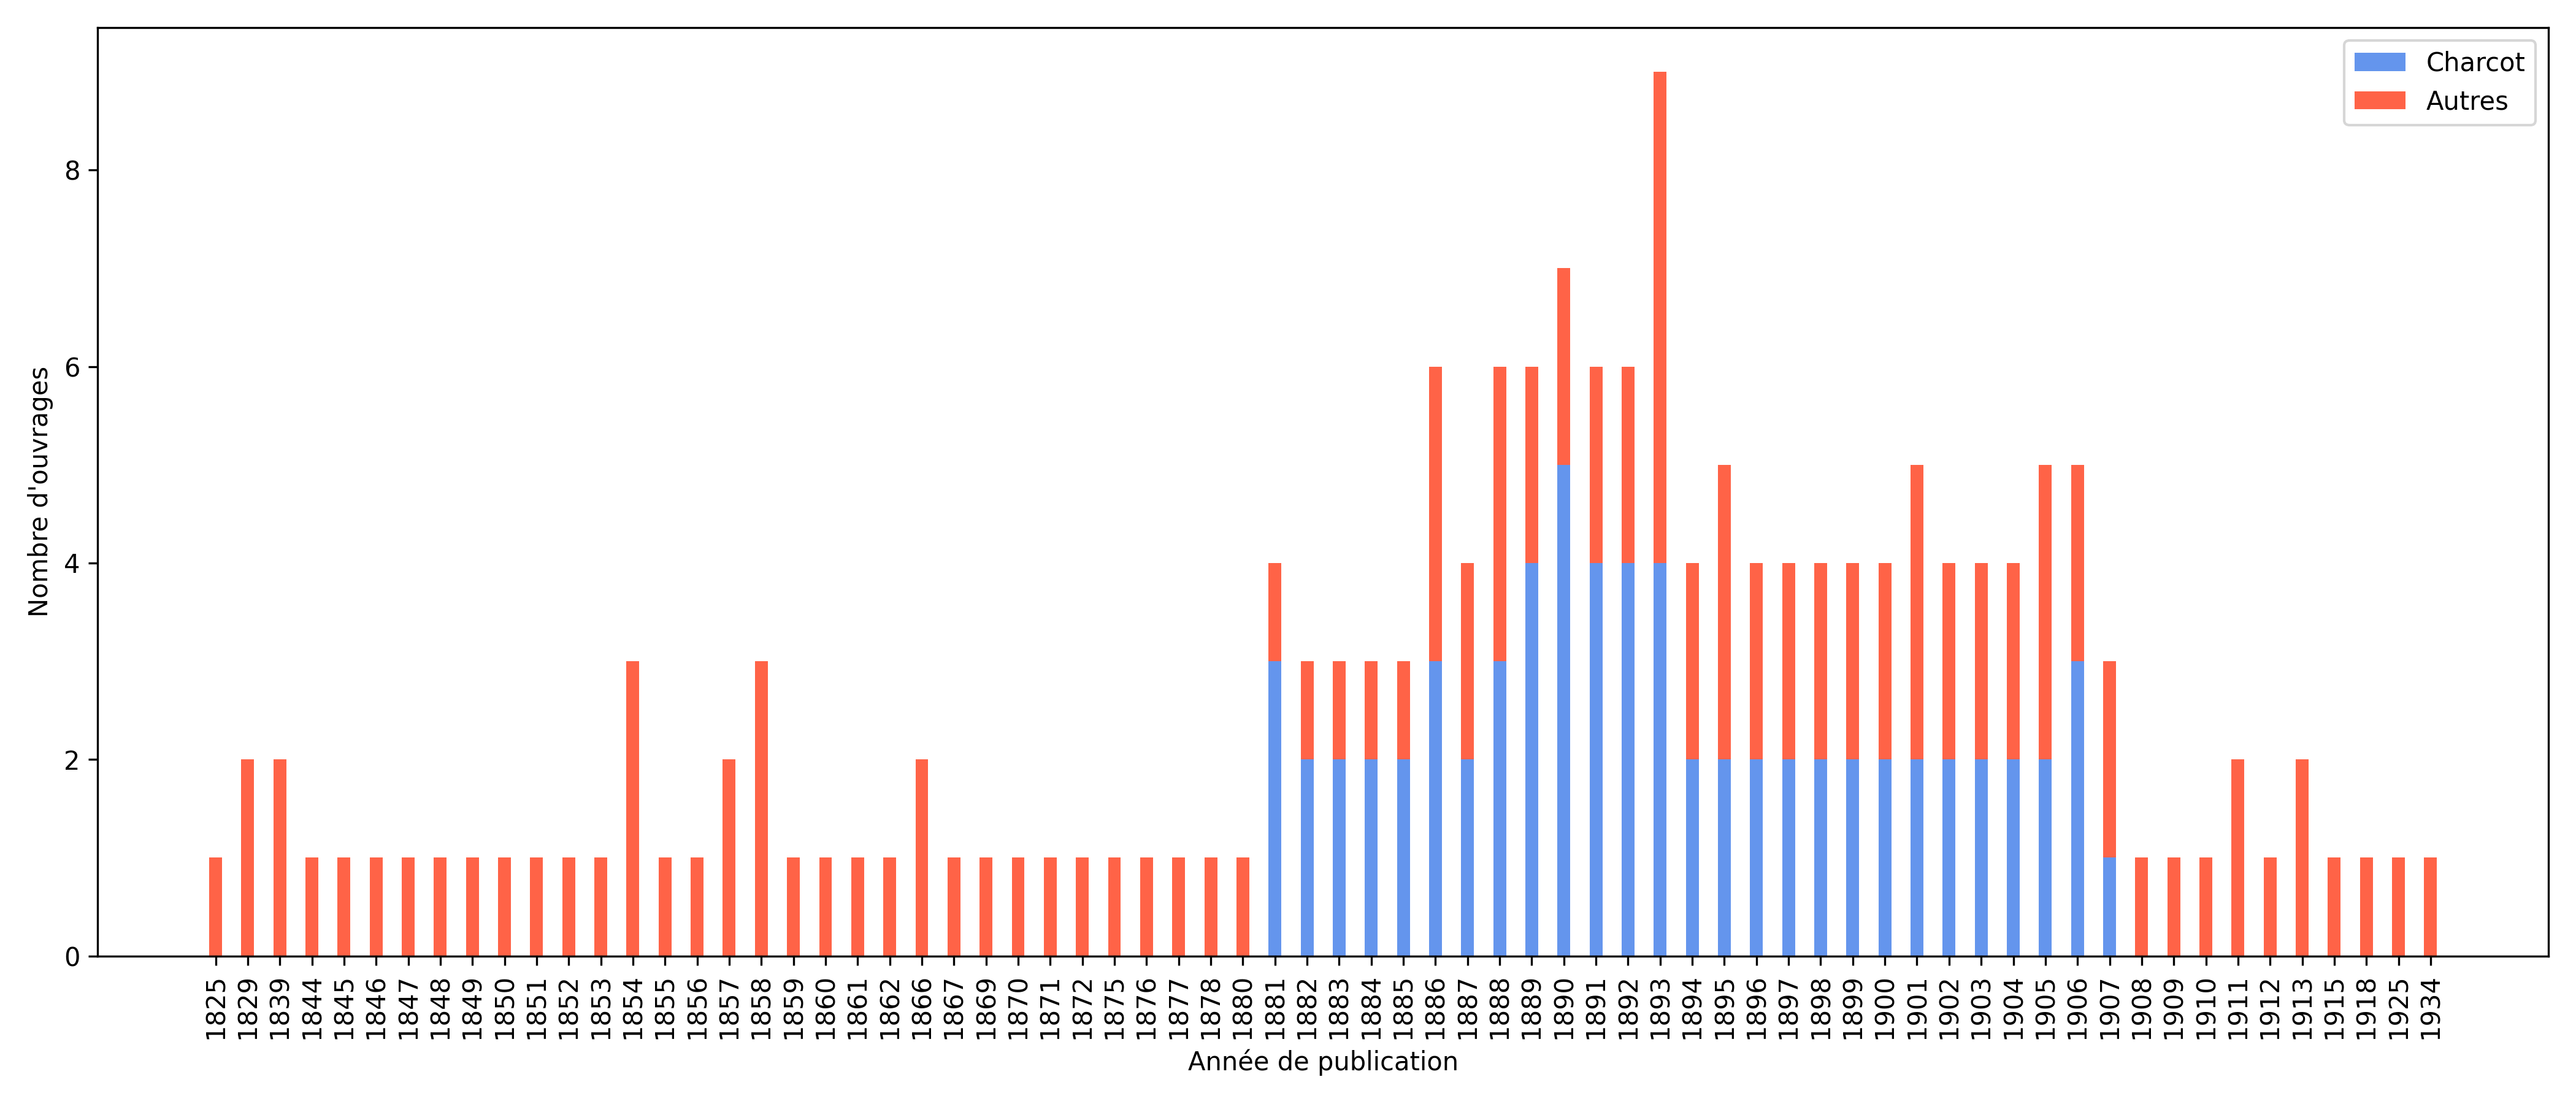
\includegraphics[width=1\textwidth]{img/distribution_ouvrages.png}
	\caption[Positionnement de l'entité \texttt{Jean-Martin Charcot} au sein de son domaine et comparaison avec les entités les plus similaires à lui \textit{via} une analyse de quadrant de l'outil Rankingdom.]{Répartition des ouvrages de Charcot et des Autres par année.}
	% Pour raison de visibilité, l'image originale a été agrandie, ce qui a entraîné le rapprochement des années sur l'axe de l'abscisse.
	\label{fig:analyse_quadrant}
\end{figure}


\section{Historique de l'\textsc{ATR}}